% This is "sig-alternate.tex" V2.1 April 2013
% This file should be compiled with V2.5 of "sig-alternate.cls" May 2012

\documentclass{sig-alternate-05-2015}

\usepackage{listings}
% remove Copyright
\makeatletter
\def\@copyrightspace{\relax}
\makeatother

\begin{document}

\title{Requirements Engineering and Software Architecture in the Linux Kernel}
\subtitle{[Paper for the Requirements Engineering and Software Architecture course at University of Stuttgart 2015/16]}

\numberofauthors{3}
\author{
    \alignauthor Julian Kuhn\\
        \affaddr{University of Stuttgart}\\
        \email{kuhjulian@web.de}
    \alignauthor Friederike Kunze\\
        \affaddr{University of Stuttgart}\\
        \email{rixx@cutebit.de}
    \alignauthor Oliver R{\"o}hrdanz\\
        \affaddr{University of Stuttgart}\\
        \email{roehrdor@outlook.com}
}

\maketitle

\begin{abstract}

This paper tries to detail both the requirements engineering process and the general software architecture of the Linux kernel project.

With regards to the requirements engineering, the paper discusses the unusual workflow and its results within the development community.
It then continues to contrast this workflow with processes found with external contributors with their own interests in the Linux kernel development and maintenance.\\
Since all of the kernel functionalities cannot be described in this paper, we focus on the following aspects: the Virtual File System (VFS), device drivers and modules. We analyze a specific module, namely the \emph{LivePatching} module introduced in the latest Kernel release. In addition we describe the customization process of the kernel with \emph{kconfig} language and helper programs like \emph{menuconfig}.

TODO: Zusammenfassung der Resultate

\end{abstract}

% The code below should be generated by the tool at
% http://dl.acm.org/ccs.cfm
% Please copy and paste the code instead of the example below.
%
 \begin{CCSXML}
<ccs2012>
<concept>
<concept_id>10011007.10011074.10011075.10011076</concept_id>
<concept_desc>Software and its engineering~Requirements analysis</concept_desc>
<concept_significance>500</concept_significance>
</concept>
<concept>
<concept_id>10011007.10011074.10011075.10011077</concept_id>
<concept_desc>Software and its engineering~Software design engineering</concept_desc>
<concept_significance>500</concept_significance>
</concept>
<concept>
<concept_id>10011007.10010940.10010971</concept_id>
<concept_desc>Software and its engineering~Software system structures</concept_desc>
<concept_significance>300</concept_significance>
</concept>
<concept>
<concept_id>10011007.10011074.10011081.10011082</concept_id>
<concept_desc>Software and its engineering~Software development methods</concept_desc>
<concept_significance>300</concept_significance>
</concept>
</ccs2012>
\end{CCSXML}

\ccsdesc[500]{Software and its engineering~Requirements analysis}
\ccsdesc[500]{Software and its engineering~Software design engineering}
\ccsdesc[300]{Software and its engineering~Software system structures}
\ccsdesc[300]{Software and its engineering~Software development methods}

% End generated code

\printccsdesc{}

\keywords{Linux; Software Architecture; Requirements Engineering}

\section{Introduction}

% intro/relevance
The Linux kernel has, ever since its origins in 1991, changed and influenced the landscapes of software architecture and software development like few other pieces of software before and afterwards.
It has also steadily gained popularity on a variety of platforms ranging from microcontrollers over desktop computers and servers to supercomputers.
The Linux kernel is to be found nearly everywhere, and understanding both its design patterns and development process means understanding one of the most influential software projects in the history of software engineering.

% history
Its architecture as well as its development process as they exist at the moment are the result of a long history of experimentation of which the blind ends are just as instructional as the provisional result.

The Linux kernel's architecture has been called into question from the very beginning, when Linux creator Linus Torvalds and operating system expert Andrew Tanenbaum had passionate debates about the advantages and disadvantages of microkernels and monolithic kernels.
More recent examples of architectural changes would include the removal of the so-called "big kernel log" in 2011.

In comparison, the development process might seem unchanged because it still relies primarily on mails and mailinglists for communication and development.
But while the communication medium might not have changed significantly, the strict and unyielding development process existing now is a result of many years of experience with an ever-growing project with uncountable amounts of prospective contributors and features.
Preventing feature-bloat and ensuring code quality while still allowing room for new features has always been a goal of the kernel community, and its realization differs from most other software projects, either free or commercial.

% motivation

Sometimes, the structure or the processes of the Linux kernel project might seem strange or only applicable for projects of comparable size and contributor base.
But especially due to its size, history and changes this paper aims to examine the Linux kernel and establish why and how some of its structures were chosen and if they were effective in the way they were intended.

% structure of this paper … irgendwie müssen wirs ja strecken

Because of the amount of contributors, users, code and work put into the Linux kernel project, there have been various papers published, the relevant of which will be discussed in the following section.
Afterwards we will first discuss the requirements engineering process and general workflow within the Linux kernel project and its more commercial branches.
Next we  will describe ``Linux as a product line'' which is achieved by the Kconfig feature modeling language and helper tools like \emph{menuconfig}. We are focusing on the modularity aspect of the kernel, and are therefore describing the Virtual File System(VFS) which is an abstraction layer for file systems, device drivers, which are needed in order to use peripherals for example, and \emph{modules}, which can be seen as containers making it possible to provide file system implementations or device drivers as loadable components during the runtime for the kernel. 
Finally we will sum up our findings and present our conclusions regarding the software architecture and requirements engineering within the Linux kernel.

\section{Related work and sources}

One of our primary sources was the \texttt{Documentation} directory in the Linux repository itself.
On the one hand, it holds valuable and up-to-date documentation of many Kernel modules and is therefore helpful to determine the overall project structure.
On the other hand it also serves as a first point of contact for new developers and contains detailed and beginner-friendly information on the contribution process.

There are multiple secondary sources giving insight into the Linux kernel development, such as ``Understanding the Linux kernel''\cite{bovet2005understanding}, ``Linux kernel development"\cite{love2010linux}, ``Maintainability of the Linux kernel"\cite{schach2002maintainability} and ``Linux Device Drivers"\cite{Corbet:2005:LDD:1209083}.


\section{Requirements Engineering}

The following sections will discuss the requirements engineering process in the Linux kernel project, and, since the Linux way of requirements engineering is not too well-defined, will also expand upon the contribution process in general.
We will highlight the differences between both of these processes within the Linux kernel community and the software industry and try to present the consequences of the choices the Linux kernel community has made.

\subsection{Requirements engineering process}

The requirements engineering process of the Linux kernel project as it exists now is nearly non-existent beyond the quality requirements which are met by the workflow described below.
This is obviously very unusual: In the software development industry, requirements engineering is a self-evident necessity, as illustrated by the related IEEE tutorial\cite{thayer1997software} and other extensive literature on the subject.
Even other open source projects tend to have some sort of explicit requirements engineering, sometimes by way of a defined API, or community-designed requirements or even requirements imposed by a committee.

The Linux kernel project rejects all of these ways of requirements engineering.
While it does provide a large and mostly stable API externally, the documentation very explicitly states that the internal API is not and does not aim to be stable and thus does not provide requirements in itself.
Linux also is not certified with any kind of interface-related certification such as the POSIX certification group which provides a common standard for operating system interfaces, which is only used as a guideline. POSIX certified systems include OS-X and Solaris.

\subsubsection{Requirements engineering developments}

Historically, Linux development has always rather followed the demands arising from within the development community than some specific requirements.
This started at the very beginning, when Linus Torvalds was mostly focussed on getting the initial kernel to run on his own hardware and work for his own needs, which was then extended by other developers with different hardware and additional needs.

This has not changed fundamentally, as changes are still contributed by community developers following only the requirements placed upon them by the contribution process described below.
The major difference between the beginnings of Linux and the current development community is that as of 2015, more than \(80\%\) of Linux kernel developers are paid for their work on the Linux kernel\cite{corbet2015linux}.
This implies that while the requirements engineering process within the community is still unstructured, there might be less visible requirements engineering processes in external interest groups, directing their developers to work on features of their interest.

\subsubsection{External requirements engineering}

The implication that a lot of requirements engineering is happening in external corporations to align development with their own interests leaves us with something of a black box regarding requirements engineering, since there is no easy way to gain insight into corporate processes of a large amount of companies.

The most involved companies in the Linux developer community are Red Hat and Intel with a combined sponsoring of about \(20\%\) of the source tree changes.
These are two very different companies with supposedly very different goals.
Red Hat actually uses Linux as their main product, selling business and support licenses for their own Linux operating system, so where their focus within the kernel development lies is difficult to ascertain except by analysing all commits they sponsored.
Intel on the other hand is the most influential semiconductor and microprocessor producer in the world, recently also expanding towards graphics chips and other integrated hardware.
It is therefore logical to assume that Intel would be mostly concerned with kernel drivers, making sure their hardware is as well supported as it can be to give them an edge on the Linux market.

Since there are no ways to prove these assumptions for certain or even provide sources without large amounts of analysis, we decided leave our analysis of the requirements engineering process at this point and moved on to the contribution process.

\subsubsection{Comparison with common requirement engineering strategies}

As mentioned above, the internal requirements engineering process of the kernel community is nearly non-existent and therefor hard to compare with any common requirement engineering strategies.
On the other hand, the external requirement engineering processes are for the most part opaque for researchers because they are confined to the decision-making of a corporation.
In the end, we don't have enough of a process in the internal community and not enough insight into the external corporations to make a meaningful statement about the decision-making process with regards to either of the two groups.

\subsubsection{Requirements engineering results}

What we can say for certain is that the unorthodox way of handling the requirements of a large operating system kernel seems to work, and work well at that.
Linux has a overwhelmingly large share in the supercomputer market and is also primarily used for administrating servers.
Within the last ten years, Linux has also moved to the consumer Desktop with the help of Canonical's Ubuntu and is already very present in the budding market of the Internet of Things via small devices like the Raspberry Pi.
While there have been bugs and vulnerabilities within the Linux kernel, all of them have been fixed quickly after being published and none of them have exposed an architectural flaw requiring a re-write of critical kernel components.

So in summary of the few actual facts regarding the requirement engineering process, it is split between the public community and private corporations, where the public process is unorthodox and simplistic, while the different company's processes and goals are opaque and difficult to ascertain.

\subsection{Contribution process}

The contribution process and workflow of the Linux kernel is a very strict construct that has grown over time and serves two primary goals.
On the one hand it is used both to give structure to the contributions of thousands of developers, many of which contribute not very often or maybe even only once and thus have no knowledge of conventions and responsibilities beyond anything found in the official documentation.
On the other hand, a strict contribution process also serves as a way of bringing quality control to the large amounts of commits, developers, features and lines of code.

When a developer wants to change a feature or fix a bug in the Linux kernel, there are many rules they need to follow, all of them documented in the kernel software repository itself as well as many places on the internet.

First, they need to make themselves familiar with the overall structure of the Linux kernel and find the submodule they are interested in.
Every submodule has a submodule maintainer who will be the point of contact for the new developer.
Next, they need to learn the kernel coding style, also detailed in the kernel documentation, because non-compliant changes will not even be considered to be merged into the kernel.

After completing these first steps of familiarising themselves with their new environment, they may now add their feature or fix their bug and post their first design of the fix to a relevant mailing list for feedback.

The next step is generating a patch and submitting it to their subsystem maintainer after implementing feedback gained on other ways (mailing lists, colleagues etc).
The patch itself should be in the form of one or several git commits in a very specific format, specifically with very verbose commit messages detailing the goals and decisions made in the implementation, and never containing too much or too little change.
Every commit needs to be signed by the author and then has to be sent to the subsystem maintainer, again in a very specific mail format, using only plain text and most commonly only one commit per mail.

After some time of consideration, the subsystem maintainer will provide feedback to the developer, who needs to apply the feedback to his patches and re-submit them.
This can be repeated as often as the subsystem maintainer is not willing to accept the patch.

Once the patch is accepted, the original developer does not have to do anything anymore, but his patch is not yet in the mainline kernel.
For this to happen, the subsystem maintainer will sign the commits again, to indicate his knowledge and approval of the patch, and submit them to either another maintainer or Linus Torvalds himself during the next merge window.
A merge window is said to be open at the beginning of every development cycle.
During this time, sufficiently stable patches are accepted and merged into the main kernel branch.
After the merge window closes, the kernel is tested to assure that all patches work and every component works well with the others.
During this time, only security patches and patches of glaring bugs are accepted.
Only when this period of testing is finished, too, the original patch will be published to the public Linux kernel.

\subsubsection{Quality control}

Quality control happens at at least two large points of control during this process.
The first is the subsystem maintainer, who needs to sign off all changes and will be held accountable for any errors.
Subsystem maintainers are chosen for their experience and reliability and skill.
It is possible to ask for the expertise of others at this point if the subsystem maintainer feels that they cannot decide if a change is stable or correct.
Since sometimes a subsystem maintainer will report to another maintainer, this adds even another point of quality control, since no maintainer would just merge changes into their branch without checking it for quality issues.

The second point of quality control is the testing happening before a release.
Linux has a lot of ways of testing kernel versions, among them large amounts of regression tests and later on many dedicated testers who run unstable Linux kernel versions on their own hardware.
During the testing period, kernel versions are published weekly, and it takes about six to ten weeks until a new stable kernel version is released.
Since the goal of releasing a new kernel version is to have all regressions fixed before the release, and there is no fixed timeframe to be adhered to for a release, Linux testing and quality control is unusually thorough.


\section{Software Architecture}
\subsection{Overview}
Since from the very first release of the Linux kernel in August 1991 \cite{linuxtimeline} with about 150.000 lines of code, the current version has grown to over 15 million lines of code. In order to manage this huge amount of code, a sophisticated architecture is needed.
\begin{figure}[h]
\centering
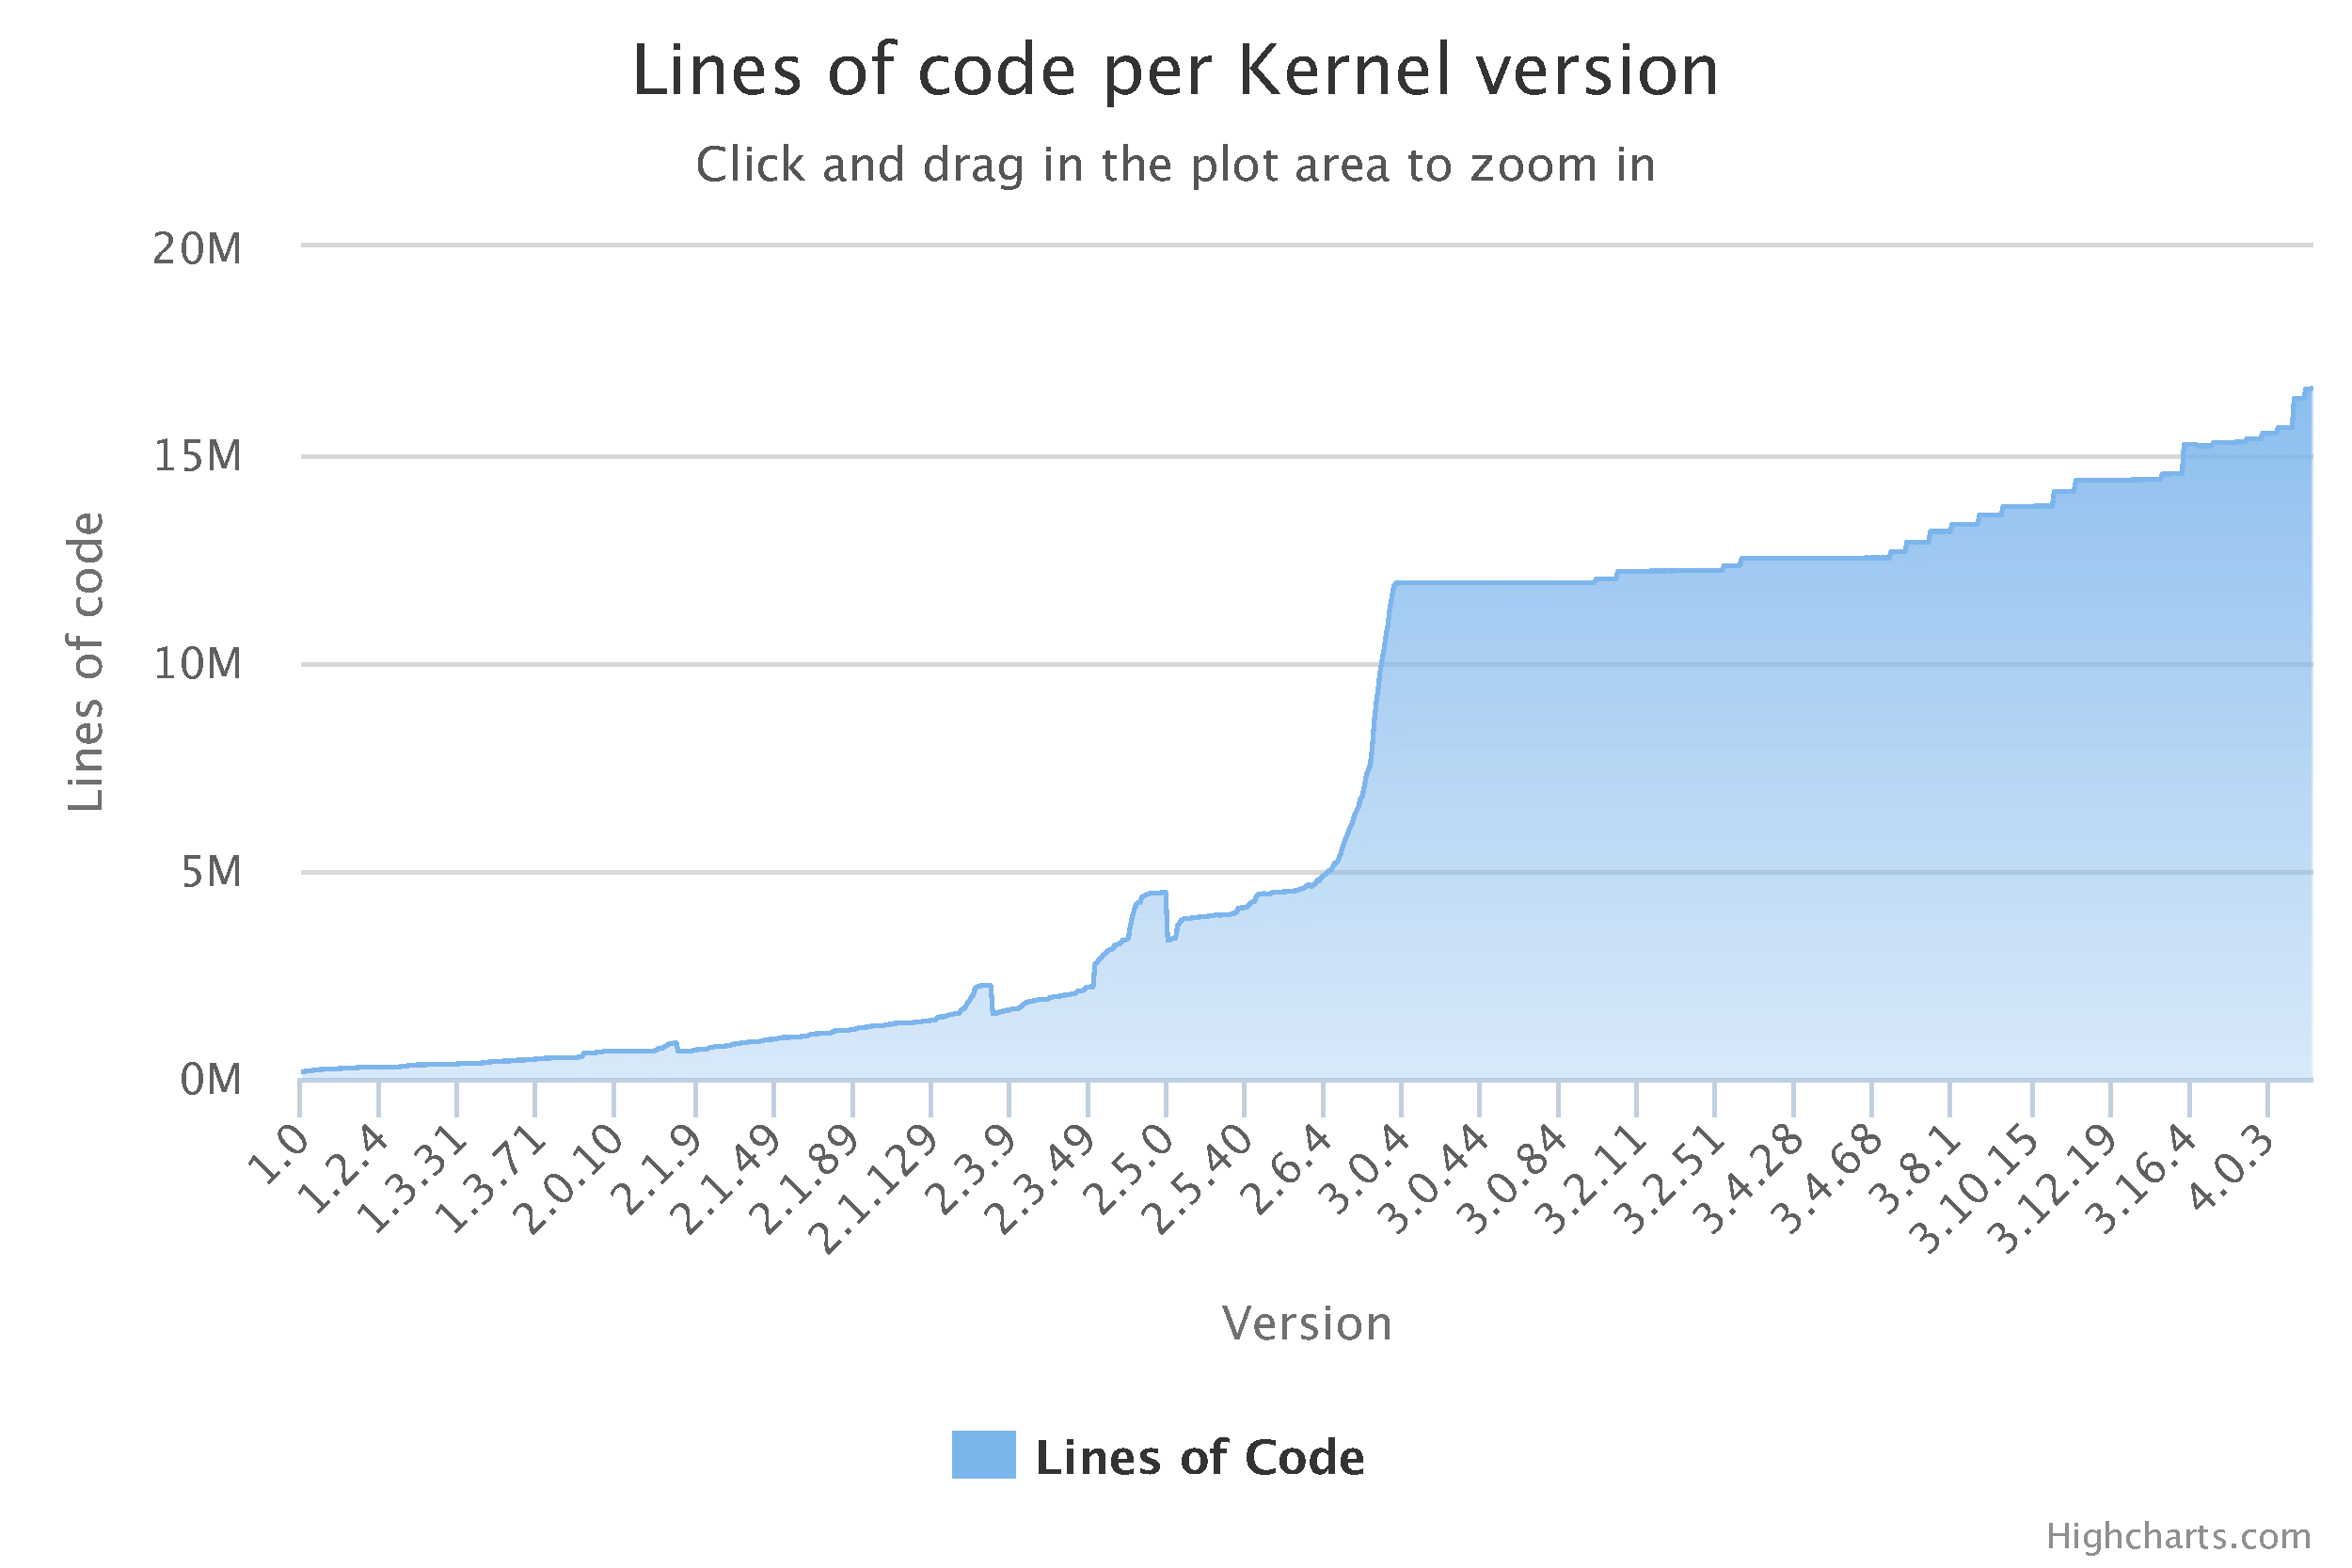
\includegraphics[width= 0.45\textwidth ]{img/chart.pdf}
\label{kconfig-compil}
\caption{Evolution of lines of code of the Linux kernel \cite{linuxcounter}}
\end{figure}

Additionally, there must be an easy way to include and exclude features from a kernel image. 
Figure \ref{fig:kernelmap} shows overview of the Linux kernel. Among other main features, the kernel provides the following  components \cite{mauerer2010professional}:
\begin{figure}[h]
\centering
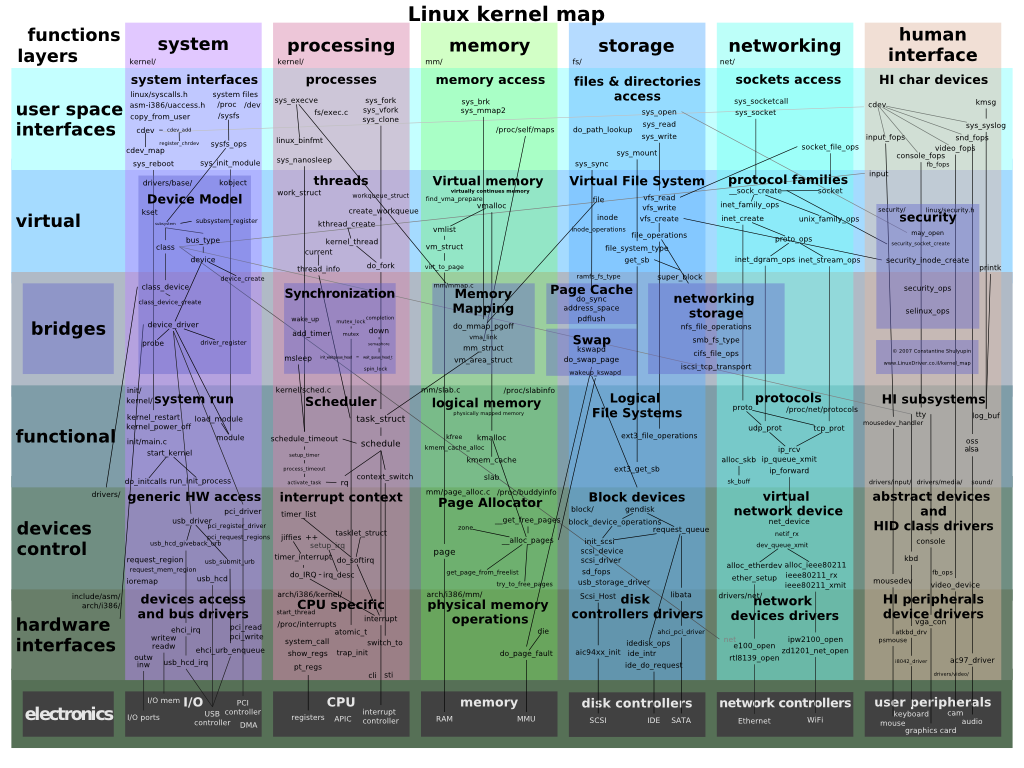
\includegraphics[width= 0.45\textwidth ]{img/Linux_kernel_map.png}
\label{fig:kernelmap}
\caption{"Linux kernel map" by Conan at English Wikipedia \cite{kernelmap}}
\end{figure}


\begin{itemize}
\item \emph{Virtual Memory}: The kernel separates the virtual address space into a kernel and user address space. Both spaces need to be managed and mapped to physical memory.
\item \emph{Virtual File System}: In order to provide support for a large variety of file systems, the kernel uses an abstraction layer called virtual file system (VFS).
\item \emph{Networking}: Linux also supports the  Internet protocol suite \cite{almquist1992type}, making it one of the larges features of the kernel by comprising around 15 MB of source code alone.
\item \emph{Device drivers}: In order to  support e.g. peripherals, device drivers are needed to use them. The Linux kernel uses an abstraction layer, supporting different categories of device drivers.
\item \emph{Process scheduling and threading}: To support multitasking and quasi parallelism, extensive process managing and the support of threads are needed.
\item \emph{System Call Interface} As there is an separation between the user and kernel space, an interface to the kernel space is needed. The System Call Interface provides functionalities, executed in the kernel space that are callable from the user space.
\end{itemize}


Because it is impossible to cover all topics visualized in figure \ref{fig:kernelmap}, we will focus on a small part and cover the following topics in this chapter:
\begin{itemize}
\item \emph{Linux as a product line}: We will describe the Kconfig language and how users can customize a kernel image.
\item \emph{Virtual file system}: The VFS is an abstraction of file systems. Here we will focus on read operations and how they are implemented if one wants to develop a new file system support for Linux.
\item \emph{Device drivers}: Device drivers are an essential part of every operating system. We will shorty describe the types of device drivers supported by Linux and give a brief introduction on how device drivers can be developed.
\item \emph{Modules}: Modules can be seen as containers for System Calls, file systems or device drivers. We briefly give an introduction on how modules can be developed and what tools can be used to integrate them into the system.
\end{itemize}


\subsection{Monolithic vs Microkernels}
Most operating systems separate the virtual memory into two address spaces: the kernel space and the user space \cite{stankov2006discussion}. Processes running inside the kernel space are for example allowed to access memory spaces of other processes. This makes these processes fast and unrestricted yet introducing a security risk if one can get unauthorized access to one of these processes. Therefore, most of the processes are running inside the user space, which gives the process lots of restrictions. For example, these processes are only allowed to access their own memory space. \\
Microkernels isolate their core functionality, which is running in kernel space, from other services or drivers. File systems for example are running in user space. Communication is taking place with explicite message passing (IPC). The advantage of this approach is, that every system service running in user space can be just restarted in the case of a failure. The problems microkernels are having is that they are difficult to debug because of the IPC message passing \cite{le2005gnu}. \\
In opposite, a monolithic kernel runs all device drivers, the file system or networking in kernel space and these function blocks are coupled tightly. 
So the terms \emph{monolithic kernel} and \emph{microkernel} refer to the amount of functionality they are providing in kernel space.\\
Linux is a modular, monolithic kernel. In addition to the fixed kernel functionalities compiled into the kernel image, Linux provides so called Loadable Kernel Modules (LKMs). The LKMs extend the functionality of the Operating System and they can be loaded and unloaded into the kernel space dynamically during runtime. By using Modules,  many advantages of the microkernel architecture can be achieved \cite[pp. 11]{bovet2005understanding}. In Chapter \ref{chap:mods}, we will focus on LKMs. \\


\subsection{Linux as a product line}
As stated above, the Linux Kernel has an monolithic architecture, forcing the user the compile a new kernel image if features should be added or removed static kernel. Of course, these customization would be impossible, if the user himself had to configure the makefiles or sources.\\
To provide a standard way of preconfiguring the integration of features into the image. A feature modeling language, called Kconfig \cite{kconfig} is used for this purpose. In the following, we will describe how the kconfig language works and how the configuration is reflected into makefiles.
\subsubsection{Configuration Process}
Kconfig is a feature modeling language developed for the Linux kernel compilation. Kconfig is used since Kernel version 2.5 \cite{mauerer2010professional}. In the following, the syntax and main components of the Kconfig language will be described.\\ Each directory of the kernel sources has its own kconfig file. The top-level kconfig files are including the child-configuration files and merge them together.\\ Inside the Kconfig files, the corresponding sources and dependencies are described. If a user wants to view and select features, he can use a program like menuconfig. Through this program, all configuration files are read and a tree structure according to the dependencies and the directory structure is built. The user can select/unselect the features he wants to add to the kernel. These selections are then stored into a separate ``.config'' file. This file is then used for the custom compilation.\par 
\subsubsection{Kconfig language}
The kconfig language uses a hierarchical structure to describe configurations. The top-level element is called ``menu''. Inside this declaration, attributes and configuration options are declared. \\
\emph{Configuration options} always begin with the keyword ``config'' and are followed by a symbol. After that, declarations of different types can be made. The available types are ``bool, ``string'', ``hex'', ``integer'' and ``tristate'', except the last one, all types are the same as from other  common programming languages. ``Tristate'' refers to three states : ``y'', ``n'', ``m'' with the meaning ``compiled in'', ``modular'' and ``do not compile''.\\
Other \emph{keywords} are ``comment'' and ``source''. The first adds a comment which is displayed to the user without a selection option. The keyword ``source'' makes a reference to other configuration files, and just copying the content of the referred files into the current one like it is done in C - language  includes.\\
\emph{Attributes} are used to describe the \emph{configuration options} in more detail. ``Default'' is setting a default value for the config entry, e.g. ``y'' or ``n'' with a bool type. ``Range'' is specifying  upper and lower borders for numeric values like int. ``Select'' is used for an automatic selection of other configuration options if that configuration is selected by the user. This can be for example used to resolve dependencies automatically.\\
The attribute ``help'' displays a helping text.''depends on'' introduces restrictions when selecting a configuration option. A option with a ``depends on'' clause may only be selected if all other dependencies are resolved. In order to describe sophisticated dependencies, logical operations `''\&\&'' and ``||'' can be used. Listing \ref{lst:kconfig} shows an example including all the previously described language details.
\lstinputlisting[frame=single,  basicstyle=\tiny, caption=Excerpt from linux/samples/kconfig, label=lst:kconfig]{lst/kconfig_example.txt}

\subsubsection{Compilation process}
\begin{figure}[h]
\centering
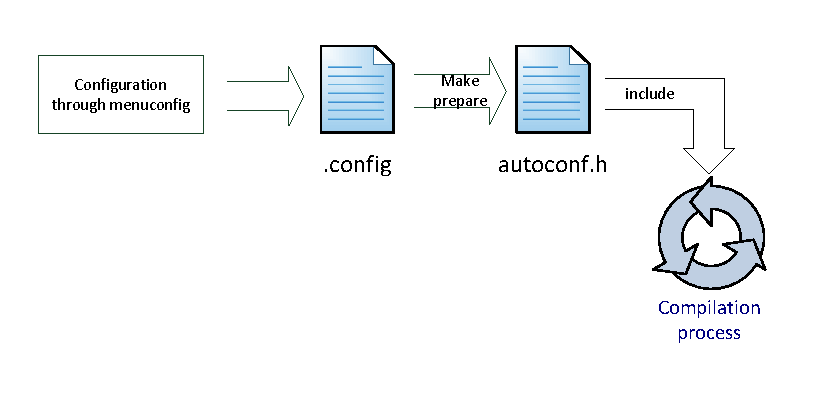
\includegraphics[width= 0.45\textwidth ]{img/kconfig-compil.pdf}
\label{kconfig-compil}
\caption{Configuration process with kconfig}
\end{figure}
Through the usage of helper programs like ``menuconfig'', which generates a tree structure out of all kconfig-files, the user can specify the features he wants to have in the kernel. All selections are saved in a separate file ``.config'' . Out of this file a c-header file is generated with the name ``autoconf.h'', reflecting the configurations as preprocessor directives. This header file is linked to the compilation of the kernel. Inside the actual source code, it will be checked if certain directives are defined. For each \#define in the ``autoconf.h'' the corresponding code part will be available for compilation. Figure \ref{kconfig-compil} illustrates this process.




%\subsection{Process Management}
%Modern Operating Systems give the user a so called pseudo-parallelism. In contrast to a single process operating system where one process must be finished before the next can start, modern operating systems will allow multiple processes to run in parallel. As this is not a real parallelism but a software implementation of parallelism, the operating system is granting every process a small portion of runtime and is assigning these time portions to the processes through a scheduling mechanism. \\
%Linux does not fulfill real-time requirements as there is no guarantee that a process may respond with a hard deadline. Since version 2.6.23 the kernel is using a completly fair scheduler. In the following, this scheduling mechanism will be described.\par
%Every process has a life cycle. A process can have the following states during its life cycle: “running”, “waiting”, “sleeping” and “stopped”. Besides of that, there can be zombie processes, which are not working correctly but still running and consuming memory.
%A scheduler is a mechanism to assign time-slices to processes. The linux scheduler is not using the traditional way of computing time slices for all processes and recalculating the time slices if they are used up. Instead, only waiting-time is considered for scheduling. The process with the largest waiting time will be scheduled next. As for the scheduling queue, a red-back tree is used. The task with the largest waiting-time is always the leftmost entry. [TODO evtl mehr auf redblack eingehen]
\subsection{Virtual Filesystem}
A operating System must support many different types of filesystems but also needs to provide a standard interface for creating,modifying and reading data on these file systems. For this purpose, a layer between the standard library (Libc) and the actual file system implementations is inserted: the Virtual File System (VFS). \\
%[TODO: bild einfuegen, dass abstraction zu konkretem FS zeigt]
The VFS abstracts  operations common to all filsystems, for example direct file operations or access controls. In the following, three small aspects of the VFS are described: the main file objects, the abstract read operation and how specific implementation aspects are reflected in the VFS.
\subsubsection{Main file objects }
There are four main file objects, namely the Superblock, Inodes,Dentries and Files. In the following, these four objects will be described in short and how they interact. 
The Superblock contains information about the file system itself and is stored on the disk redundantly. Information stored is  for example  the used/free number of blocks and the root Inode.
Files typically lie on a hard drive and have a starting block and a length. Of course, they can be divided into several blocks. There needs to be some kind of representation where the concrete data of the file lies and if it is divided into pieces. For this purpose, Linux is using Inodes. They abstract concrete files. They contain metadata of the file status, like the creation date or the permission and also pointers to the actual data. An Inode can also serve as a symbolic link to another Inode.\\
Dentries are not store on the disk, but are rather used for caching reasons. They contain the name of the file, a pointer to the inode, the parent dentry and child dentries. Dentries resemble the tree structure of the file system in memory and are used to increase performance.
File(-objects) represent currently opened files and contain information like the current data pointer inside the file, the size and the mode. Like dentries, they are not stored persistently.\par
The following scenario visualized in figure \ref{fig:vfs-bsp} shows the interaction between the main objects of the VFS:
\begin{figure}[h]
\centering
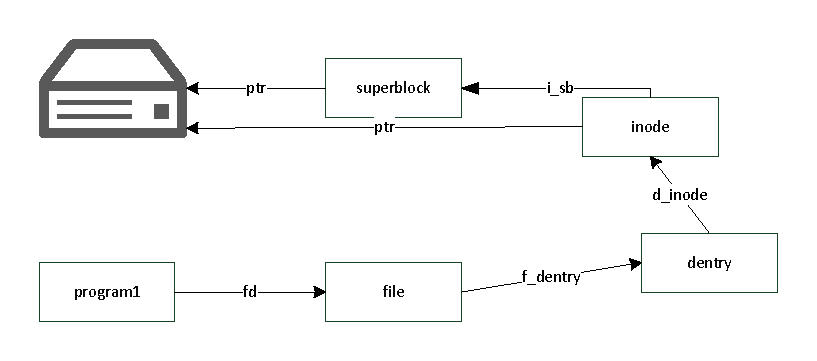
\includegraphics[width= 0.45\textwidth ]{img/vfs-bsp.pdf}
\label{fig:vfs-bsp}
\caption{Pointer structure of an opened file}
\end{figure}

Suppose a user program ``program1'' is opening a file, thus creating a file-objects containing all mode and  meta informations. The file-object has a pointer to a dentry (f\_dentry is the pointer inside the struct). The dentry itself is  pointing to the corresponding inode of the file, its superblock, and to the physical location of the data. 

\subsubsection{Abstract read operation}

If anyone wants support a new  type of filesystem, the kernel already provides some standard ways to deal with block devices for example. The most common type of a block device is a hard drive, where the physical storage is separated into chunks with a fixed length.
In the following, we will look how a read() is working when a user program has opened a file and wants to retrieve some data from the file:\\
First of all, there is a common struct called ``file\_operations'', which provides a standard way of reading,writing and other functionalities. Listing \ref{lst:file-operations} shows a small excerpt of the struct.
\lstinputlisting[language=C, basicstyle=\tiny, frame=single, caption=Excerpt of the file-operations struct, label=lst:file-operations]{lst/file-operations.c}
In order to provide custom opearation, the developer needs to declare a file\_operations struct, where he sets the function pointer to his own function. Listing \ref{lst:file-operations-ext3} shows the usage of the file-operations struct of the ext3 filesystem. 
\lstinputlisting[language=C, basicstyle=\tiny, frame=single, caption= Excerpt of the file-opeartions implementation for ext3, label=lst:file-operations-ext3]{lst/file-operations-ext3.c}

 As a filesystem could have different kind of files (e.g. directories, normal files, or named pipes) there could be the need for different kind of read functions.\\
When a file is opened, a program read or write data from it. As figure \ref{fig:vfs-read-abstraction}shows, the read operation invoked in user space actually calls  the kernel function sys\_read(). The sys\_read() function actually delegates to the vfs\_read() function which either invokes a file specific method or a generic function, called do\_sync\_read. 
The vfs\_read() function checks, if there is any specific read function is provided for this kind of file. If not, it uses the generic read function defined in the file\_operations struct.  Figure \ref{fig:generic_read} shows this procedure.
\begin{figure}
\centering
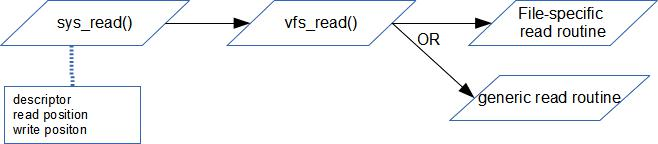
\includegraphics[width= 0.45\textwidth ]{img/generic_read.jpg}
\label{fig:generic_read}
\caption{Selection of file specific read operations}
\end{figure}

 The vfs\_read() has the filedescriptor used to identify the file, the current read position and, after reading, this position will be updated. Inside it, either the specific or generic function will be called.\\
Besides of the customizable file\_operations struct, Linux already provides a generic implementation for block-devices, which are for example used by the ext3 implementation shown in Listing \ref{lst:file-operations-ext3}. 


\begin{figure}
\centering
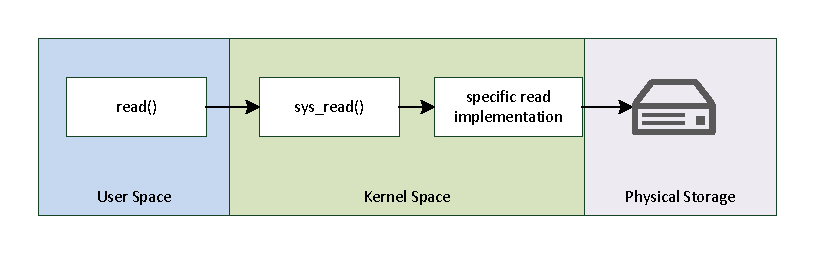
\includegraphics[width= 0.45\textwidth ]{img/vfs-read-abstraction.pdf}
\label{fig:vfs-read-abstraction}
\caption{General functionality of the abstract read operation}
\end{figure}

\subsection{Modules}
\label{chap:mods}
Besides the fixed features parts of the kernel image, which will be available immediately after the start of the system, Linux allows so called Modules to be loaded into the system during runtime. A Module can be seen as a type of container for device drivers, system calls or filesystems.
This approach has many advantages: New functionality can be deployed as a precompiled module and be loaded into the system dynamically. If new drivers are needed, users can just download and load the corresponding module. In addition, experimental features can be tested in an easy fashion without the need to reboot the system with each change of the module code.
\subsubsection{General functionality}
A Module consists of two major parts: The internal code and exported functions that can be called from userspace. A module can have dependencies to other modules. 
The following files contain information about modules:
\begin{itemize}
\item \emph{/lib/modules/<kernel version>/modules.dep}: Dependencies  between the currently used modules are listed inside this file.
\item \emph{/lib/modules/<kernel version>/kernel}: All available modules are listed here.
\item \emph{/etc/modules/modprobe.conf}: All modules listed in this file will be loaded at startup into the system.
\item \emph{/proc/modules}: Inside this file, all currently loaded module are listed.
\end{itemize}

The representation of module inside the kernel is done through a structure called \emph{module} which is defined inside \emph{module.h}. For each module which is integrated into the running system, one instance of this struct is existing. The struct contains general information about the module like the name, several function pointers for methods common to all modules, as well as the actual code providing the functionality of the specific module.

In the following, a brief description on how modules are developed are given and how they are loaded and unloaded into the system.


\subsubsection{Developing Modules}
In order to develop a module on your own, three kernel specific header files are needed in general:
\begin{itemize}
\item \emph{<linux/init.h>}: Provides several macros for registering functions.
\item \emph{<linux/module.h>}: Interface header file in order to develop modules.
\item \emph{<linux/kernel.h>}: As normal c-library functions are not available inside the kernel, this header file gives kernel specific equivalents. For example, the normal printf() function cannot be used inside modules. Instead, one can use printk().
\end{itemize}
 Listing \ref{lst:mod-example} shows a sample module source code .
An init-function will be called whenever the module is loaded, inside that, objects could be allocated for example. The init\_function returns a error code where  0 represents a success. \\
The exit-function is called when a module is unloaded. 
These functions must be registered via macros which are included by \emph{init.h}.  In addition, there are macros included from \emph{module.h} in order to mark the license of the module code. The code can be marked as GPL, several GPL mixed with BSD/MIT/MPL licences or proprietary. Also there are macros to include a description of the module, the authors, a name alias and some short info text.


\lstinputlisting[language=C, frame=single,  basicstyle=\tiny, caption=Module example code, label=lst:mod-example]{lst/module_example.c}

From the user perspective, a kernel module is compiled the same way as a normal c file. Internally the Kbuild system is used. Listing \ref{lst:mod-example} shows an example makefile.


\lstinputlisting[frame=single,  basicstyle=\tiny, caption=Example makefile, label=lst:mod-mk]{lst/makefile.mk}
Modules are loaded to the sytem as binary blobs. The binary is structured in the ELF binary format. By using this format, predefined sections can be used to include the module specific code. \\


\subsubsection{Load \& Unload Mechanism}
The \texttt{insmod} and \texttt{modprobe} functionalities can be used to load a kernel module during runtime. Where \texttt{insmod} only tries to load and start the kernel module the \texttt{modprobe} functionalty also tries to resolve all the needed dependencies required to run the kernel module, not matter whether these are indirect or recursive dependencies of the target module. \\
\texttt{insmod} copies the compiled code and module data from the userspace to the kernel space and checks for external linkage, but in comparison to a normal linker this process does not modify the module's disk file but only the temporary data that has been copied to run the module.

Modules are loaded into the kernel via the system call \emph{sys\_init\_module} which is copying the module data from the userspace into the kernel space. In addition, the system call is parsing the module for optional sections, checking if the format is correct and is processing arguments. 

Users can add modules into the system with the \emph{modprobe} and \emph{insmod} commands. Insmod inserts a single module while modprobe also takes care of dependencies between multiple modules.

\subsection{Device Drivers}
Device Drivers are an essential part of every operating system. Linux also supports device drivers. In most cases, device drivers are developed as modules in order to integrate them into the system dynamically. In the following, we give a short overview what kind of drivers can be developed and a short introduction how they are developed. 
\subsubsection{Overview}
In the view of the Linux kernel there are three different device types for which drivers can be written. These are \texttt{char modules}, \texttt{block modules} and \texttt{network modules}. Still programmers have the choice to implement different devices in the same code (driver), which is nonetheless not recommended \cite{Corbet:2005:LDD:1209083}.

\paragraph{Char modules}
A character device can be accessed in a stream fashioned way, and can be compared to accessing a file. But there are still a differences between accessing regular files and these character modules, whereas a regular file allows seeking (jumping forward or backward in the file non sequentially) the underlying stream of a character module needs to be accessed sequentially. The are some excetions where once can also seek in these character modules using \texttt{mmap} and \texttt{lseek} functions, but this ist not usually the case. The driver is responsible to implement this behavior and therefore needs to at least implement the \texttt{open}, \texttt{close}, \texttt{read} and \texttt{write} system call operations. Some examples for a character module are \texttt{/dev/console} or \texttt{/dev/ttyS0}. These character devices can be accessed through nodes in the filesystem, usually in the \texttt{/dev} directory.

\paragraph{Block module}
As the char device a block device is also accessed through the \texttt{/dev} file system directory and normally represents a device that hosts a filesystem. Most Unix Operating Systems do not allow working with single bytes here, instead they work with block sizes. A block is usually a 512 bytes large chunk of data (can also be more, needs to be power of 2). Linux in comparison allows a block device also to work at byte and not just at block leven. So the difference between a block device and a character device is rather small and differs only in the way the data is represented internally in the kernel since they have a completely different interface to the kernel than char drivers. A example for a block device is the hard drive of the system.

\paragraph{Network module}
Network connections are made through interfaces, an interface can be a pure software device, e.g. such as loopback devices or real hardware devices that can actually exchange data with different hosts. Despite many network connections are stream-oriented the network driver does not need to know anything about the connection it has been involved in. The network driver is only responsible of sending and receiving packets. \\
In comparison to the block and character driver a network driver is not easily mapped to a node in the filesystem, a character device could be accessed as \texttt{/dev/console}, what is not possible for network devices since they are not a stream oriented device. Instead the linux driver assigns unique identifiers and names to these intefaces, for network devices the probably best known one is \texttt{eth0}. Instead of using the known \texttt{open}, \texttt{close}, \texttt{read} or \texttt{write} system calls a network devices uses kernel functions that are completely related to packet transmission. 

\subsubsection{Developing Device Drivers}
On the one hand device drivers can be added statically to the Linux kernel, but this is only useful im some scenarios, e.g. when the system always needs a specific driver to work and this driver is already needed a startup, another scenario would be an embedded system, where the hardware is actually known and stays the same for the whole time. \cite{Corbet:2005:LDD:1209083} \\

\paragraph{Security}
In our modern times security is getting more and more important, although a driver programmer should avoid encoding security policies in their own code. The security policies are often and best handled by the kernel itself, if the knerl has any security holes in it, the whole system may be vulnerable. Still there are some rules a programmer should follow to ensure the system and driver is working.
\begin{itemize}
\item A driver that deals with input from the user should be suspicious. one should always assume the user wants to crash and hurt the system, therefore the input should never be trusted. It is also important to deal with uninitialized memory, in case this is done wrong data leakage might occur and important data might be compromised. To develop such a driver the author needs also to assure the user can not input any data that can harm the system.
\item Since the kernel is written in the C programming language also the modules and the drivers are written in C. Unfortunately C makes it easy to introduce a lot of common programing error such as buffer overruns or reading or writing into invalid memory. Thes errors can compromise the stability of the whole system and should be definately prevented.
\item A device driver should also be aware that in some cases some types of devices could affect the system. Some devices need to access global ressources which could actually damage the hardware physically or that could affect other users. Functions to set the default block size of a tape drive for example should only be done from privileged users, this check is not done by the kernel but needs to be done by the driver developer himself.
\end{itemize}

Writing a device driver is not that different from writing a kernel module. By loading the module into the kernel memory, some preliminary tasks need to be performed, these tasks are reserving RAM, interrupts and resetting the device. These tasked are permored by the kernel functions \texttt{module\_init} and \texttt{module\_exit} previously described. 


\subsection{Live Patching}
Since Linux ist used as a server operating system as well as on regular desktops and mobile devices, developers strive to maximze the reliability, therefore minimizing the mean time between failures and maximizing the uptime of the service. So far updates to the system have really been critical, since the system was not able to adopt software changes on the fly, but therefore required some maintenance time for applying those. These maintenance times always involved some down time of the service. Many companies applied those security and feature updates in the night time when the service usage has been quite low. This has been working so far but also lead to problems in security since the server ran the faulty software for several hours being vulnerable to zero-day attacks. \\
These issues led several companies such as SUSE and Red Hat to develop and introduce kGraft and kpatch in early 2014. Two kernel live patching technologies which aim to solve two problems \cite{kgraft-1}, incident response on the one site and emegency change on the other hand. The feature of live patching has been merged into the linux kernel mainline in late 2014 combining most of the features of kGraft and kPatch, which are pretty similar in its functionality.

\subsubsection{kGraft}
A kGraft patch itself is also just a kernel modul and has been implemented with only a small amount of code, since this module uses a lot of other leveraging linux technologies. To allow changes to the executed code on runtime kGraft makes heavy use of the insmod command, which installs a loadable modul into the running kernel, and therefore does not need to stop the running kernel. To make this technology work kGraft needs some additional space at the beginning of functions to modify them at runtime, this can be achieved by using gcc's \texttt{-pg} compiler flag which inserts a special function call at the beginning of functions which can later be used by kGraft to route around faulty functions, meaning data structure changes can not be patched and inserted into an running kernel at runtime. To redirect the code flow kGraft also uses this extra space like ftrace, this space is exactly 5 bytes, which is replaced with \texttt{NOP} instructions by the kernel at boot time. When the code flow needs to be redirected kGraft inserts a \texttt{INT3} instruction into the first byte, the following four bytes are filled using destination address. Finally the first byte is replaced again now containing a \texttt{JMP} instruction.

\begin{figure}[ht!]
	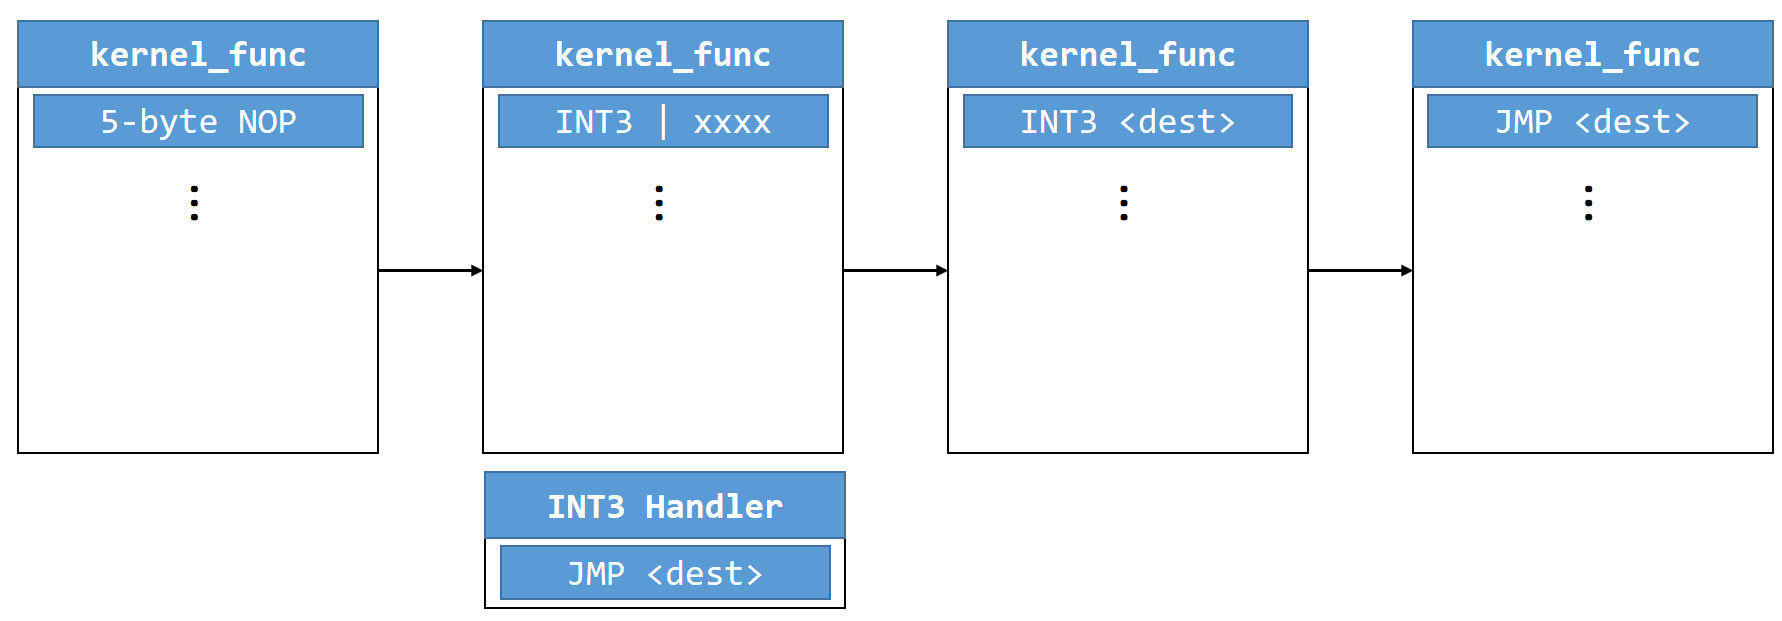
\includegraphics[width=0.5\textwidth]{img/kgraft_code_reflow.png}
	\caption{Code reflow \cite{kgfraft-1}}
	\label{fig:kgraft-code-reflow}
\end{figure}

The caller has not to change anything, the whole code reflow procedure has been completely done at function level, which justs redirects the function call to itself to a new, probably patched version of the exectuable code. \\ 
\\
But kGraft is now just limited to redirect the existing code flow but also provides the functionality to insert new functions and methods that shall be added to the kernel at runtime, still without the need to call \texttt{stop\_kernel()} and still without patching the anything of the caller's code.

\begin{figure}[ht!]
	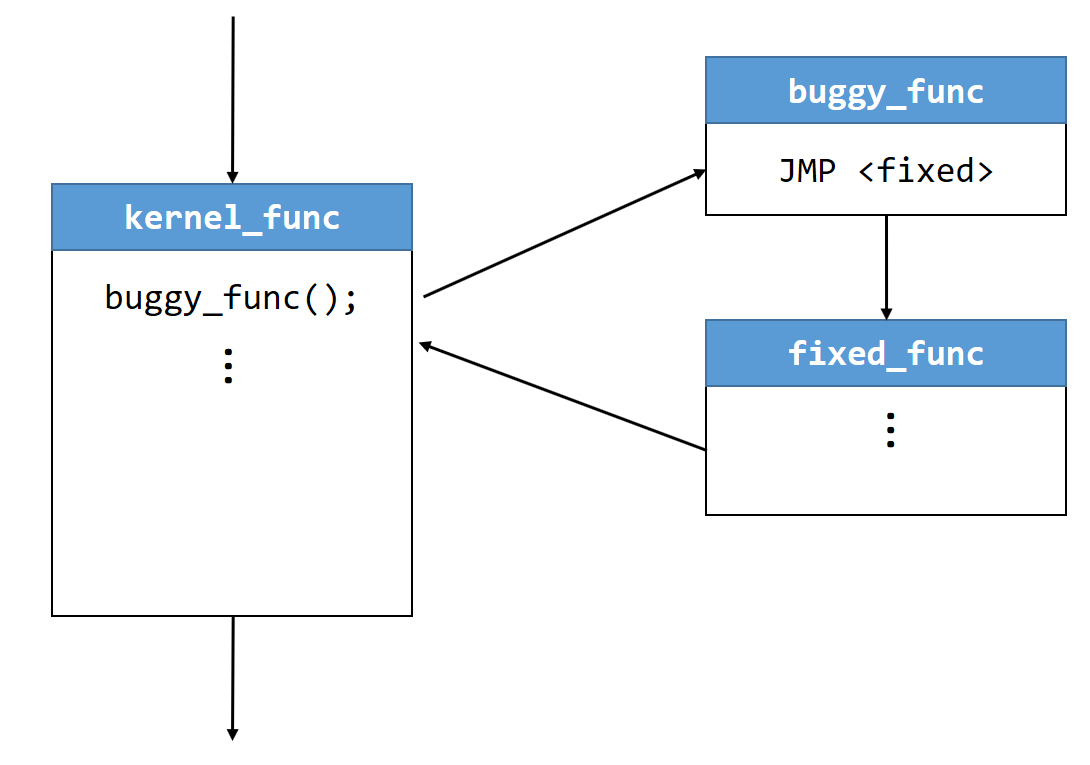
\includegraphics[width=0.5\textwidth]{img/kgraft_new_func.png}
	\caption{New function \cite{kgfraft-1}}
	\label{fig:kgraft-new-func}
\end{figure}


\begin{figure}[ht!]
	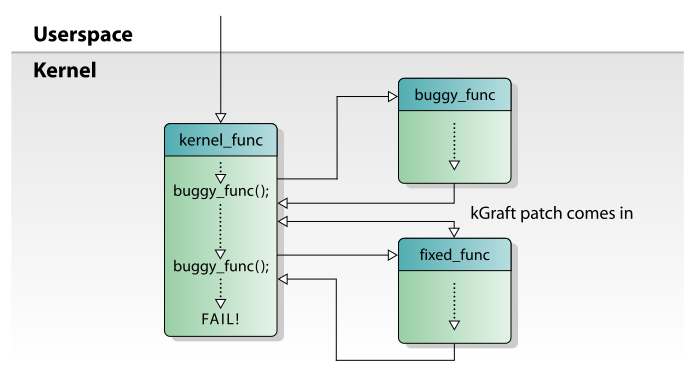
\includegraphics[width=0.5\textwidth]{img/kgraft-live-patching-realty-check-1.png}
	\caption{Fail without reality check https://en.wikipedia.org/wiki/KGraft}
	\label{fig:kgraft-real-check-fail}
\end{figure}

Inserting a new function is not that different from just redirect the code flow. Again the first bytes of the function are used, which are replaced with a \texttt{JMP} instructon to the address of the new, fixed function that needs to be executed. \\ Still there may be unresolved issues, Figure~\ref{fig:kgraft-real-check-fail} shows a scenario where the same function is called twice during a single system call or kernel function execution. The same fail might occur when calling the function recursivly. There needs to be a check which of these functions, the faulty or the patched one, has been used the first time so that the same function is used again to provide consistency in the system call. These function need to use the same data structures but may access them differently and therefore using both of the functions will probably result in kernel crash. In the final implementation the RCA algorithm has been used to keep consistent views of the to be patched or already patched functions. This algorithm implements kind of a mutlual exution with a low overhead and wait free read events, only the updates might be expensive  \\
Therefore kGraft also does some reality checks, therefore each process is monitored and ensured to execute the same function, either still the old or already the new one consistently within the same, single system call. After everything has finally migrated to the new version these reality checks are no longer needed and do not need to be executed anymore. 

\subsubsection{kPatch}
kPatch is pretty similar to kGraft described above, it also aims to implement live patching. It also works at function level and uses the functionalities provided by ftrace to route around the function and to redirect the executed code flow \cite{kpatch}. kPatch has the same limitations, it is possible to change the code but not to change the kernel data structures. Since these live patching systems are primarly desinged to apply security patches on the fly, which rarely change the kernel's data structure this is an acceptable limitation.



%%
%% Conclusion
%%
\section{Conclusions}

TODO: Conclusions



\bibliographystyle{abbrv}
\bibliography{sigproc}  % sigproc.bib is the name of the Bibliography in this case
%  and remember to run:
% latex bibtex latex latex
% to resolve all references

\balancecolumns{}
\end{document}
